
\section{Detektorempfänger}
\label{section:detektorempfänger}
\begin{frame}%STARTCONTENT

\begin{columns}
    \begin{column}{0.48\textwidth}
    \begin{itemize}
  \item Einer der ersten und einfachsten Empfänger für AM
  \item Energie wird direkt aus dem empfangenen Signal gezogen
  \item Nur im Lokalbereich von starken Rundfunksendern nutzbar
  \end{itemize}

    \end{column}
   \begin{column}{0.48\textwidth}
       
\begin{figure}
    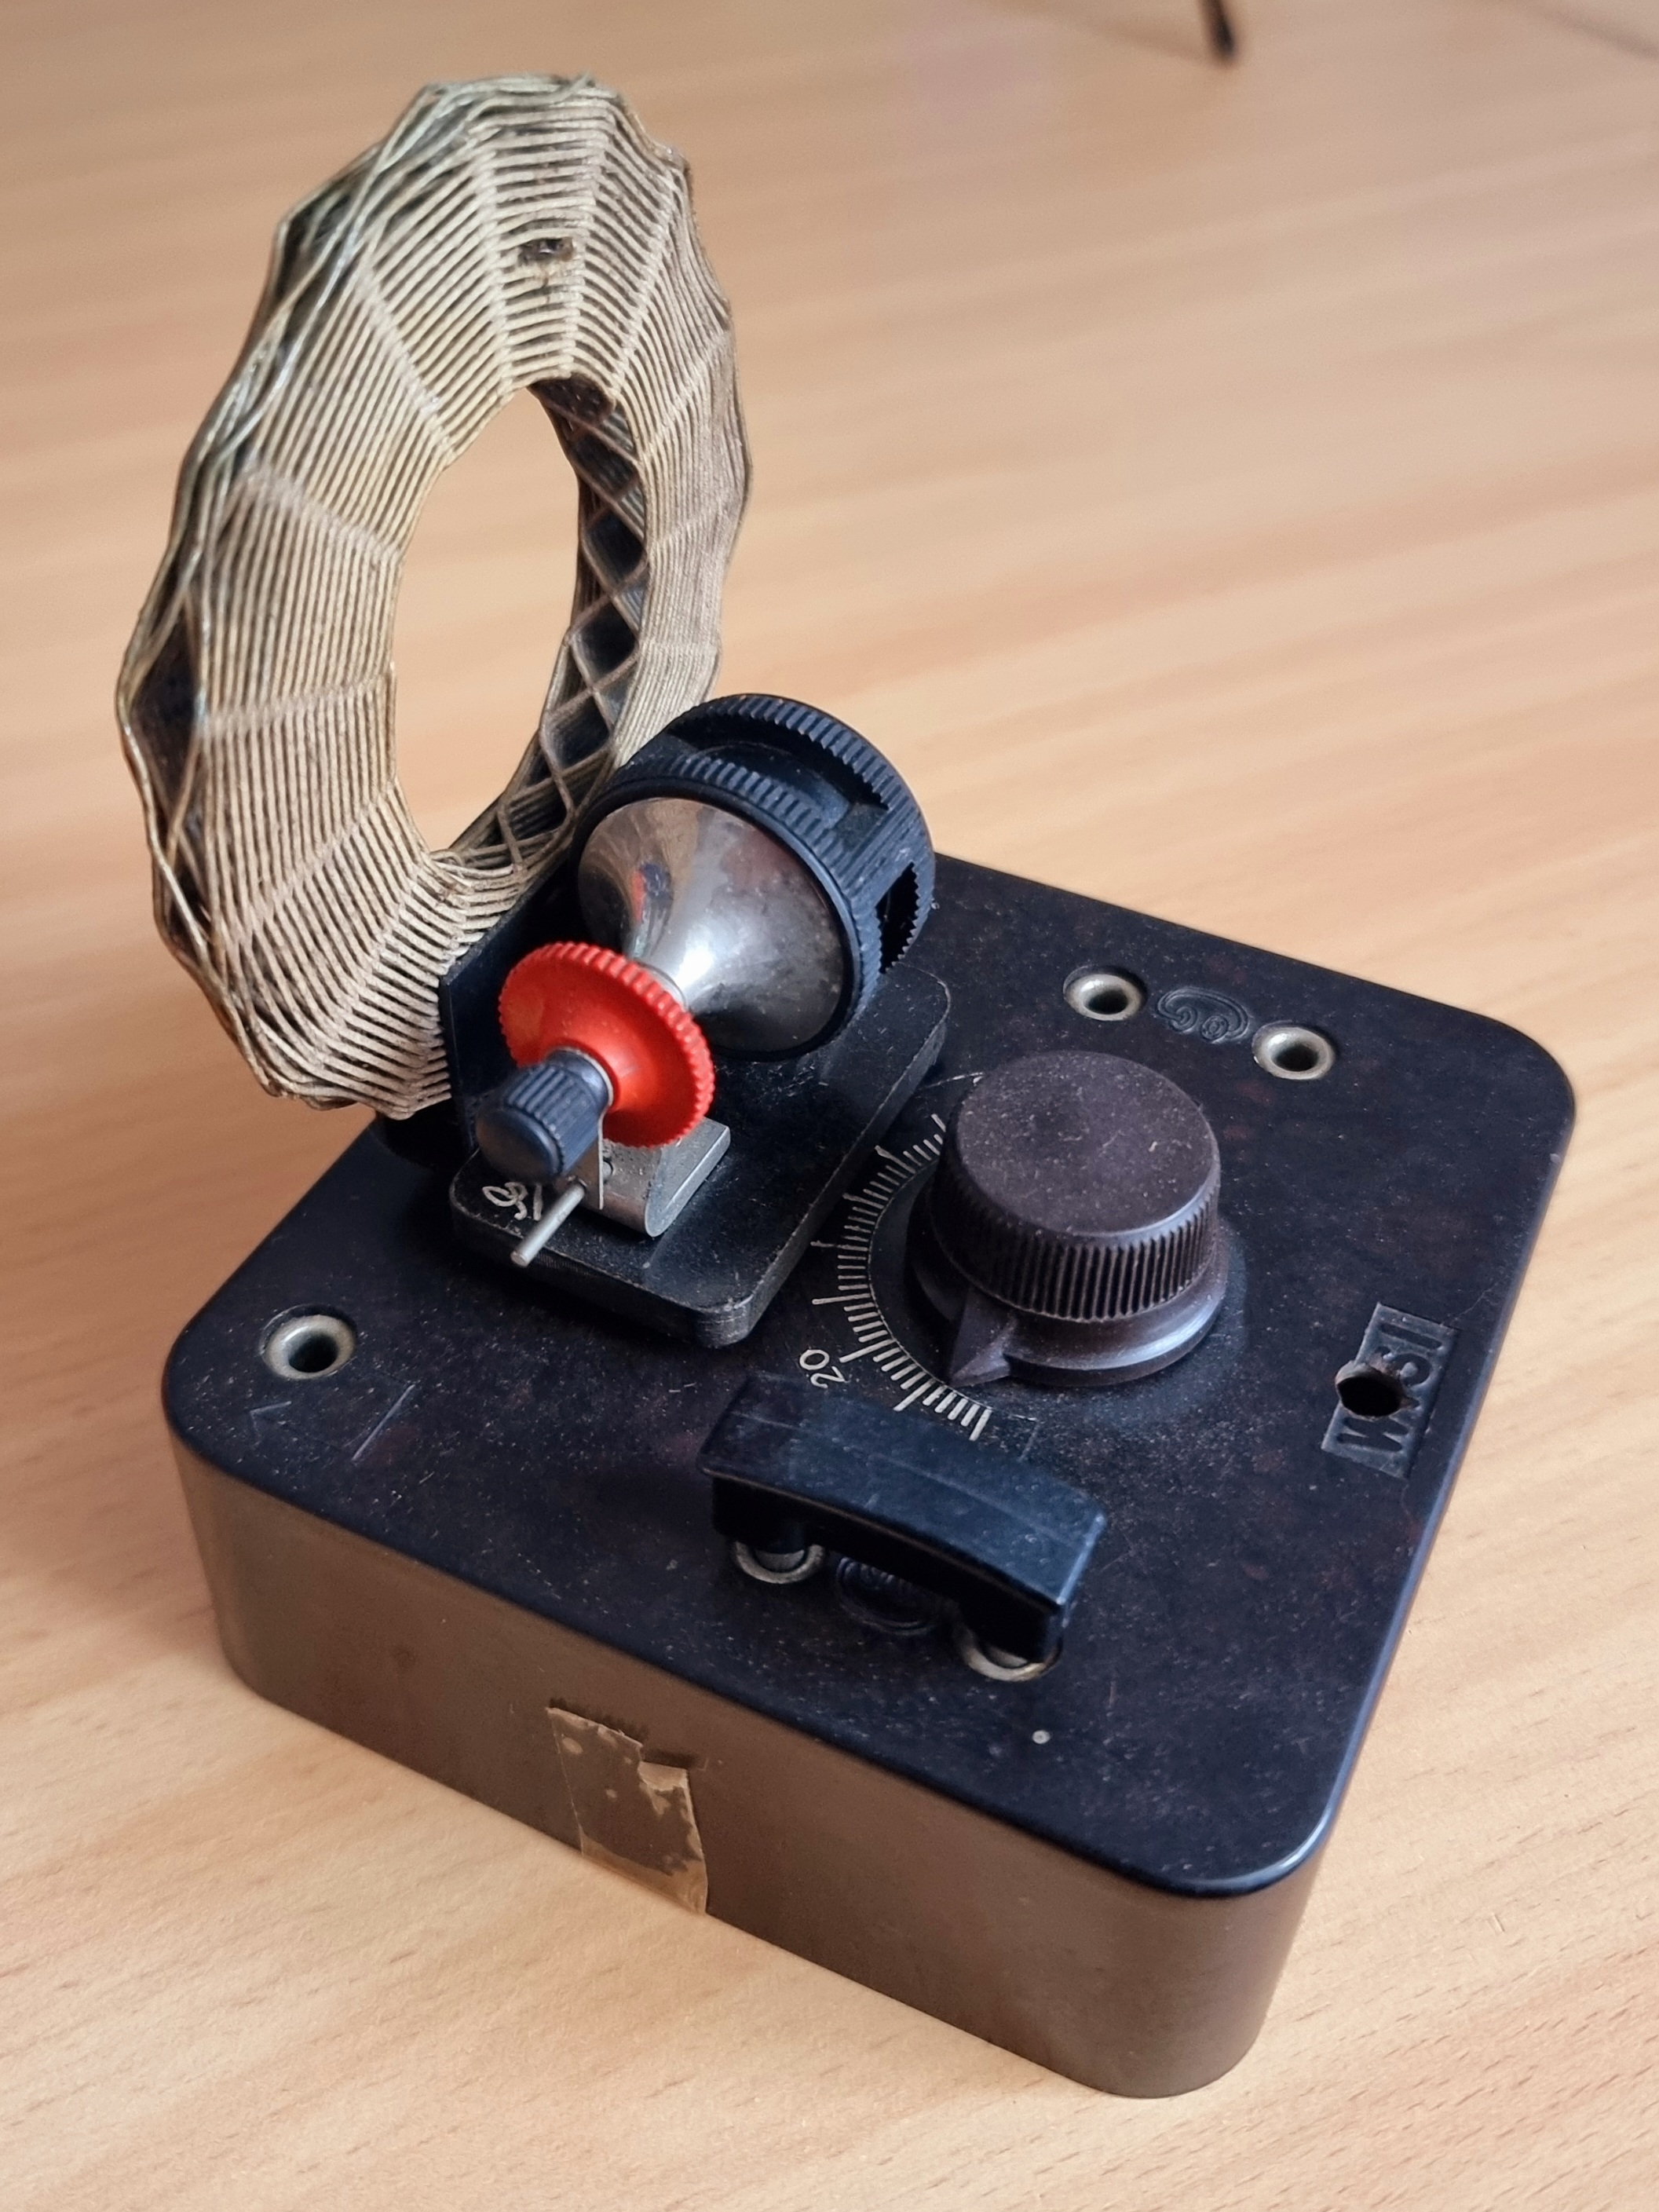
\includegraphics[width=0.85\textwidth]{foto/193}
    \caption{\scriptsize Detektor-Empfänger}
    \label{am_detektor}
\end{figure}

   \end{column}
\end{columns}

\end{frame}

\begin{frame}
\begin{columns}
    \begin{column}{0.48\textwidth}
    
\begin{figure}
    \DARCimage{0.85\linewidth}{799include}
    \caption{\scriptsize Schaltbild eines einfachen Detektor-Empfängers}
    \label{am_detektor}
\end{figure}

\begin{itemize}
  \item Parallel-Schwingkreis aus Spule und variablen Kondensator
  \end{itemize}

    \end{column}
   \begin{column}{0.48\textwidth}
       
\begin{figure}
    \DARCimage{0.85\linewidth}{800include}
    \caption{\scriptsize Signal an der Antenne}
    \label{am_detektor_antenne}
\end{figure}


\begin{figure}
    \DARCimage{0.85\linewidth}{801include}
    \caption{\scriptsize Gleichgerichtetes Signal an der Diode}
    \label{am_detektor_diode}
\end{figure}


\begin{figure}
    \DARCimage{0.85\linewidth}{802include}
    \caption{\scriptsize Hörbares NF Signal}
    \label{am_detektor_kopfhoerer}
\end{figure}


   \end{column}
\end{columns}

\end{frame}

\begin{frame}
\begin{columns}
    \begin{column}{0.48\textwidth}
    
\begin{figure}
    \DARCimage{0.85\linewidth}{799include}
    \caption{\scriptsize Schaltbild eines einfachen Detektor-Empfängers}
    \label{am_detektor}
\end{figure}

\begin{itemize}
  \item Signal von Antenne (rot) regt Schwingkreis an, wenn dieser auf die Frequenz abgestimmt ist
  \end{itemize}

    \end{column}
   \begin{column}{0.48\textwidth}
       
\begin{figure}
    \DARCimage{0.85\linewidth}{800include}
    \caption{\scriptsize Signal an der Antenne}
    \label{am_detektor_antenne}
\end{figure}


\begin{figure}
    \DARCimage{0.85\linewidth}{801include}
    \caption{\scriptsize Gleichgerichtetes Signal an der Diode}
    \label{am_detektor_diode}
\end{figure}


\begin{figure}
    \DARCimage{0.85\linewidth}{802include}
    \caption{\scriptsize Hörbares NF Signal}
    \label{am_detektor_kopfhoerer}
\end{figure}


   \end{column}
\end{columns}

\end{frame}

\begin{frame}
\begin{columns}
    \begin{column}{0.48\textwidth}
    
\begin{figure}
    \DARCimage{0.85\linewidth}{799include}
    \caption{\scriptsize Schaltbild eines einfachen Detektor-Empfängers}
    \label{am_detektor}
\end{figure}

\begin{itemize}
  \item Diode (blau) richtet die AM-Modulation gleich
  \end{itemize}

    \end{column}
   \begin{column}{0.48\textwidth}
       
\begin{figure}
    \DARCimage{0.85\linewidth}{800include}
    \caption{\scriptsize Signal an der Antenne}
    \label{am_detektor_antenne}
\end{figure}


\begin{figure}
    \DARCimage{0.85\linewidth}{801include}
    \caption{\scriptsize Gleichgerichtetes Signal an der Diode}
    \label{am_detektor_diode}
\end{figure}


\begin{figure}
    \DARCimage{0.85\linewidth}{802include}
    \caption{\scriptsize Hörbares NF Signal}
    \label{am_detektor_kopfhoerer}
\end{figure}


   \end{column}
\end{columns}

\end{frame}

\begin{frame}
\begin{columns}
    \begin{column}{0.48\textwidth}
    
\begin{figure}
    \DARCimage{0.85\linewidth}{799include}
    \caption{\scriptsize Schaltbild eines einfachen Detektor-Empfängers}
    \label{am_detektor}
\end{figure}

\begin{itemize}
  \item Hochohmiger Kopfhörer (grün) macht das Signal hörbar, da der Kopfhörer träge ist und den einzelnen Stromstößen nicht folgen kann
  \end{itemize}

    \end{column}
   \begin{column}{0.48\textwidth}
       
\begin{figure}
    \DARCimage{0.85\linewidth}{800include}
    \caption{\scriptsize Signal an der Antenne}
    \label{am_detektor_antenne}
\end{figure}


\begin{figure}
    \DARCimage{0.85\linewidth}{801include}
    \caption{\scriptsize Gleichgerichtetes Signal an der Diode}
    \label{am_detektor_diode}
\end{figure}


\begin{figure}
    \DARCimage{0.85\linewidth}{802include}
    \caption{\scriptsize Hörbares NF Signal}
    \label{am_detektor_kopfhoerer}
\end{figure}


   \end{column}
\end{columns}

\end{frame}

\begin{frame}
\only<1>{
\begin{PQuestion}{EF101}{Was stellt nachfolgende Schaltung dar?}{Modulator}
{Verstärker}
{Oszillator}
{Detektorempfänger}
{\DARCimage{1.0\linewidth}{523include}}\end{PQuestion}

}
\only<2>{
\begin{PQuestion}{EF101}{Was stellt nachfolgende Schaltung dar?}{Modulator}
{Verstärker}
{Oszillator}
{\textbf{\textcolor{DARCgreen}{Detektorempfänger}}}
{\DARCimage{1.0\linewidth}{523include}}\end{PQuestion}

}
\end{frame}%ENDCONTENT
